\section{BP on a grid}
\label{app:bp}

\note{Grid $g_i=-A+(i-1)h$, $A=8$, $\Ng=401$, $h=0.04$, trapezoid weights $w_i$; kernel matrix
$K_{ij}=K(g_i\mid g_j)$ (arrival $i$, origin $j$); $\ell_k(i)=\ell_t(x_k\mid g_i)$. The two sweeps, the posterior
mean, the pair posteriors and the log-likelihood from the forward normalisers.}
\begin{gather*}
  f_1=\mu\odot\ell_1,\qquad f_k\propto\ell_k\odot K(w\odot f_{k-1});\qquad
  \beta_L=1,\qquad \beta_k\propto K^{\top}(w\odot\ell_{k+1}\odot\beta_{k+1});\\
  \E[a_k\mid x]\approx\frac{\sum_i w_i g_i f_k(i)\beta_k(i)}{\sum_i w_i f_k(i)\beta_k(i)}.
\end{gather*}

\label{app:numerics}
\begin{figure}[h]
  \centering
  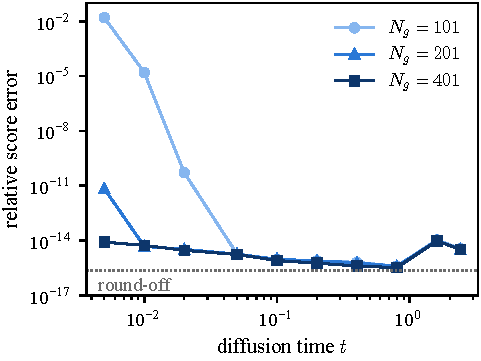
\includegraphics{fig_grid_gaussian}\hfill
  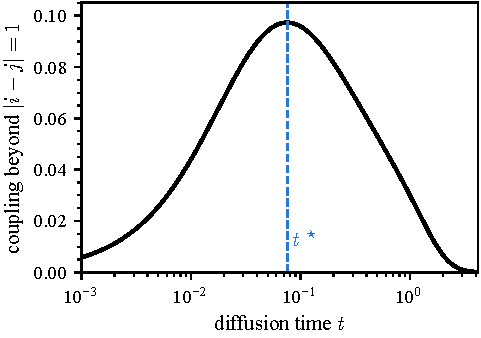
\includegraphics{fig_locality_curve}
  \caption{Left: grid BP against the exact score $-Q_tx$ on the Gaussian chain ($\alpha=0.8$) for three grid sizes;
  the dotted line is double-precision round-off. Right: coupling of $Q_t$ beyond nearest neighbours, relative to the
  nearest-neighbour coupling of $Q_0$, against $t$; it peaks at $t^\star$.}
  \label{fig:grid}
\end{figure}

\section{EM: M-steps}
\label{app:em}

\note{Closed forms: Gaussian AR(1) (posterior-weighted Yule--Walker), Laplace AR(1) (weighted median), mixture (ECM),
log-linear families (concave $Q$, gradient = observed minus expected), neural energy (autograd on $Q$, GEM: a few
Adam steps per iteration, step halved when $Q$ does not increase). Checkpoint ladder and selection rule.}

\begin{figure}[h]
  \centering
  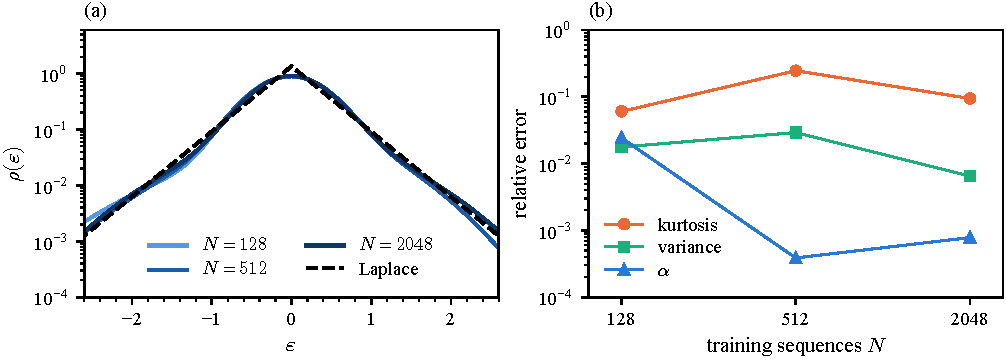
\includegraphics{fig_em_innovation}
  \caption{Mixture kernel ($C=8$). (a) Learned innovation law against the Laplace truth. (b) Relative error of
  $\alpha$, of the innovation variance and of its excess kurtosis against $N$, one fit per $N$.}
  \label{fig:em-innovation}
\end{figure}

\section{Sources of error}
\label{app:errors}

\note{J\'er\^ome: the error decomposition goes here. Grid (quadrature and truncation), kernel misspecification,
finite data, EM stopping. Thesis Ch.~7--8.}

\section{Network baselines}
\label{app:networks}

\note{Six architectures, parameter counts, hyperparameter screen, training recipe (DSM on clean sequences, Adam,
checkpoints at 500--32{,}000 steps, validation selection), the pairing with EM--BP on the same test sequences (E02a and
E03).}

\section{Allen--Cahn details}
\label{app:field}

\note{Cells (temperature, spacing, correlation), the family definitions (site energy, tilted spline, log-linear 2-D,
MDN, shift mixture), the networks, and the $M=128$ table.}

\begin{table}[h]
  \caption{As \cref{tab:field}, from $M=128$ training sequences.}
  \centering
  \small
  \begin{tabular}{@{}lcccc@{}}
    \toprule
    $\Theta$ & 0.3 & 0.5 & 1 & 2\\
    \midrule
    site energy          & 0.139 & 0.269 & 0.534 & 0.630\\
    tilted spline        & 0.218 & 0.454 & 1.110 & 1.478\\
    log-linear 2-D       & 0.385 & --    & 1.337 & --\\
    MDN                  & 0.468 & 0.900 & 1.724 & 2.457\\
    shift mixture        & 1.018 & 1.039 & 1.187 & 1.278\\
    best network         & 0.829 & 2.339 & 4.150 & 5.787\\
    \bottomrule
  \end{tabular}
  % src: ~/Code/Thesis/jerome-call-2026-10-29-slide15.md, M = 128 table
\end{table}
